\documentclass[12pt,fleqn]{article}\usepackage{../common}
\begin{document}
Destek Vektor Makinalari (Support Vector Machines)

En basit halleriyle SVM'ler risk minimize eden lineer siniflayicisidirlar. 

\[ R(\Theta) \leq J(\Theta) = R_{emp}(\Theta) +
\sqrt{ \frac{h \times (log(\frac{2N}{h}) + 1) - log(\frac{\eta}{4})}{N}}  \]

\textbf{h}: siniflayicinin kapasitesi 

\textbf{N}: egitim verisinde kac veri noktasi oldugu

Vapnik ve Chernovenkis $1-\eta$ olasilikla ispaladi ki ustteki denklem dogrudur. 
SVM algoritmasi hem $h$ degerini hem de sayisal, olcumsel riski ayni
anda minimize etmektedir, ve bunu sinir noktalarini noktalarini
ayirmakla yapmaktadir.  

Turetelim

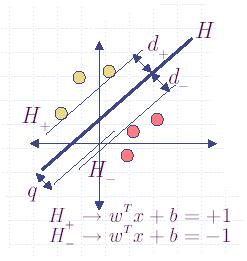
\includegraphics[height=6cm]{svm-planes.png}

Karar duzlemi: $w^{T}x + b=0$ 

Soyle bir tanim yapalim: $q = min_{x}\big\|x - 0\big\|$

\begin{itemize}
   \item $q$, $H^{+}$ ve $H^{-}$ formullerini ileride kullanacagiz.
   \item H icin: $q = min_{x}\big\|x - 0\big\|$ su sarta tabi $w^{T}x+b=0$
   \item Lagrange: $min_{x}\frac{1}{2}\big\|x - 0\big\|^2+\lambda(w^{T}x+b)$
   \item Gradyani alalim ($\frac{\partial}{\partial x}$) ve 0 degerine esitleyelim
   \item Biraz cebirsel numaradan sonra: $q = \frac{|b|}{||w||}$
\end{itemize}


\begin{itemize}
  \item Tanim:
  \begin{itemize}  
  \item $H^{+} = w^{T}x + b=+1$
  \item $H^{-} = w^{T}x + b=-1$
  \end{itemize}
  \item Bu tanimi genellikte bir kayip olmadan yapabiliyoruz; $b$ \&
    $w$ degerlerini hala duzeltebiliriz.
\end{itemize}

\begin{itemize}
  \item $q^{+}$ ve $q^{-}$ degerlerinin hesapla
  \begin{itemize}
  \item $q^{+} = \frac{|b-1|}{||w||}$
  \item $q^{-} = \frac{|-b-1|}{||w||}$
  \end{itemize}
  \item Ayrac o zaman soyle 
  \begin{itemize}
  \item $m=q^{+}+q^{-} = \frac{|b-1-b-1|}{||w||} = \frac{|-2|}{||w||} = \frac{2}{||w||}$
  \end{itemize}  
\end{itemize}

Ayraclarin olabildigince ayirmasini istiyorsak $m$'i arttiriz (yani
$\frac{2}{||w||}$'i maksimize ederiz), ya da $||w||$ degerini minimize
ederiz. 

Sinirlar

Veri noktalarini oyle siniflamak istiyoruz ki + ve - noktalar
hiperduzlemlerin dogru noktalarinda kalsinlar. 

\[ w^{T}x+b \geq +1, \forall y_{i}=+1   \]

\[ w^{T}x+b \leq -1, \forall y_{i}=-1  \]

Bu iki denklemi birlestirelim

\[ y_{i}(w^{T}x+b)-1 \geq 0  \]

Her seyi biraraya koyalim

\[ min \frac{1}{2}{||w||^2} \textrm{ subject to }  y_{i}(w^Tx_{i}+b)-1 \ge 0 \]

Bu form tanidik geliyor mu? Bu qp ile cozulebilecek karesel
(quadratic) bir formul, programdir!

qp


\begin{itemize}
   \item Python dilinde cvxopt paketi vardir
   \item Matlab Optimization Toolbox'da qp() var.
   \item Steve Gunn'in SVM Toolbox'i icinde C ile yazilmis bir qp var
   \item SVMLight icinde ayrica bir qp var
   \item qp fonksiyonlari problemleri genelde
     $\frac{1}{2}x^{T}Px+q^{T}x$ formunda gormek isterler.
   \item Biraz once elde ettigimiz denklemi bu istenen formata dogru ``masajlayabiliriz''
\end{itemize}

Ikiz (dual)

\begin{itemize}
   \item SVM ihtiyaclari icin ikiz formul (dual) ile calismak daha rahattir
   \item Lagrange (tekrar) olusturalim, turevi alalim, ve sifira esitleyelim.
   \item Bunun sonucunda elimize KKT noktalari gececektir
\end{itemize}

\begin{equation}L_{p} = \frac{1}{2}||w||^{2}-\sum_{i}\alpha_{i}(y_{i}(w^{T}x_{i}+b)-1)  \label{eq:primal}\end{equation}

\[ \frac{\partial}{\partial w} L_{p} = w-\sum_{i}\alpha_{i}y_{i}x_{i}=0  \]

\begin{equation}w = \sum_{i}\alpha_{i}y_{i}x_{i} \label{eq:wdual} \end{equation}

\begin{equation}
\frac{\partial}{\partial b} L_{p} = -\sum_{i}\alpha_{i}y_{i}=0  \label{eq:cdual}
\end{equation}

\ref{eq:wdual} ve \ref{eq:cdual} denklemini asal (primal) denklem olan
\ref{eq:primal} icine koydugumuz zaman

\begin{equation}
\textrm{ Maksimize et } L_{D}=\sum_{i}\alpha_{i}-\frac{1}{2}\sum_{i}\sum_{j}\alpha_{i}\alpha_{j}y_{i}y_{j}x_{i}^{T}x_{j} \label{eq:svm}
\end{equation}

sinirlar

\[ \sum_{i}\alpha_{i}y_{i}=0  \]

\[ \alpha_{i} \geq 0  \]

qp

\begin{itemize}
   \item Bu yine qp() formunda bir problem! Sadece bu sefer
     cozecegimiz degiskenler $\alpha_i$'lar,  $x$'lar degil. 
   \item Denklem \ref{eq:svm} su forma  $\frac{1}{2}x^{T}Px+q^{T}x$ masajlanabilir
   \item Bunun yapmak icin $P_{i,j}$'ye $-y_{i}y_{j}x_{i}^{T}x_{j}$
     degerini atariz.
   \item Ve qp'yi cagiririz
   \item Sonuc bir $\alpha$'lar listesi olacaktir.
\end{itemize}

$b$ degerini hesaplamak

\begin{itemize}
   \item KKT kosulunun sebebiyle sifir olmayan her $\alpha_{i}$ icin
     ana problemde ona tekabul eden kisitlayici sart s�k�d�r (tight),
     yani bir esitliktir.
   \item O zaman sifir olmayan her $\alpha_{i}$ icin $b$'yi
     $w^{T}x_{i}+b = y_{i}$ ifadesini kullanarak hesaplariz.
   \item Sifir olmayan her $\alpha_{i}$'dan gelen $b$ yaklasik olarak
     diger other $b$'lere esit olacaktir. Final $b$'yi hesaplamak icin
     tum $b$'lerin ortalamasini almak numerik olarak daha garantidir.
\end{itemize}

Siniflayici Tamamlandi

Her yeni $x$ noktasi icin artik $sign(x^{T}w+b)$ ibaresini
siniflayicimiz olarak kullanabiliriz. $-1$ ya da $+1$ olarak geri
gelecek sonuc bize yeni noktanin hangi sinifa ait oldugunu
soyleyecektir.

Ornek ��kt�

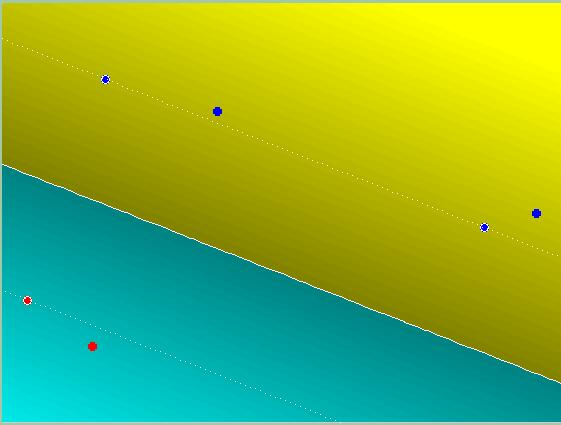
\includegraphics[height=4cm]{svmlinear.png}

Kernels

\begin{itemize}
   \item Simdiye kadar lineer ayraclardan bahsettik.
   \item SVM'ler lineer olmayan ayraclarla da calisabilir.
   \item Cok basit: Bir temel fonksiyon kullanarak girdiyi daha yuksek
     bir boyuta dogru bir onislemden gecirirsek bunu basarabiliriz.
   \item Algoritmanin geri kalani degismeden kalacaktir.
\end{itemize}

Gayri Lineer Cekirdek

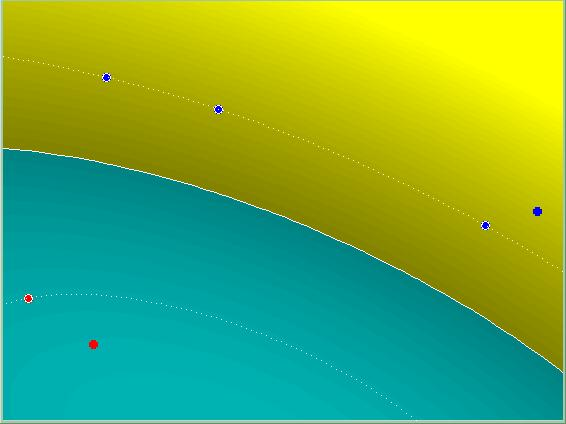
\includegraphics[height=4cm]{svmpoly.png}

Esneme Pay�

\begin{itemize}
   \item Bazen bir problem ayrilmaya musait olmayabilir.
   \item Cok uc noktalardaki bazi noktalar siniflayicinin calismasini
     imkansiz hale getirebilir
   \item Bunun cozumu icin siniflayiciya ``esneme pay�'' dahil edebiliriz.
   \item Mesela $y_{i}=+1$ icin verinin yanlis tarafa dusmesini su
     durumda izin verebiliriz: $w^{T}+b \geq -0.03$ 
   \item Fakat eklemek gerekir ki bu tur noktalarin ``cok fazla''
     olmasini da istemiyoruz, bu sebeple bu ``yanlis'' noktalarin
     sayisina da  bir ceza getirebiliriz.
\end{itemize}

\clearpage

\lstinputlisting[language=Python]{svm.py}

Not: Ikizdeki $L_d$'yi maksimize ediyoruz, fakat hala \verb!qp()!'deki
minimize ediciyi cagiriyoruz. Bu sebeple tum $\alpha$'larin toplamini
temsil eden $q$'larin negatifini aliyoruz, \verb!np.ones(n_samples) *-1! 
isleminde goruldugu gibi. Formuldeki karesel kisim icinde zaten
$-\frac{1}{2}$ negatif ibaresi var, boylece geri kalan formulun
degismesine gerek yok.

Kaynaklar

http://www.mblondel.org/journal/2010/09/19/support-vector-machines-in-python

Jebara, T., Machine Learning Lecture, Columbia University

\end{document}

